\section{Causal Consistency Models}
\label{app:cc-models}


In this appendix, we study the consistency checking problem under the \emph{causal consistency models} namely, $\ccmm, \cmmm$ and $\cvmm$ which come from distributed databases.
We begin with a brief overview of the
operational and axiomatic semantics of these models, and then show that the complexity landscape observed for the Release - Acquire (RA) variants extends to these models as well. 
Recall that for RA, we established a tight characterization of complexity with respect to the number of writer threads per memory location:
\onewriter\ admits polynomial-time
solutions, \twowriter\ is $\NP$-hard, and \threewriter\ yields a stronger
conditional lower bound. Our goal in this section is to establish analogous
results for causal consistency models, thereby showing that the same complexity results extend to $\ccmm, \cmmm$ and $\cvmm$. Next, we provide an overview of these causal consistency models. 


\subsection{Overview of Causal Consistency Models}
\label{app:cc-models-overview}

In the domain of distributed systems, causality is the key concept for consistency. There are three popular causal models, namely, Causal Consistency ($\ccmm$), Causal Convergence ($\cvmm$), and Causal Memory ($\cmmm$)~\cite{BouajjaniEGH17}. 
It is known that $\ccmm$ coincides with $\wramm$ while $\cvmm$ coincides with $\sramm$~\cite{Lahav:2022}. $\cmmm$ is stronger than $\ccmm$ and incomparable to $\cvmm$ and $\ramm$.  

In Causal Memory, each thread has a locally-consistent view of the order that different writes have been executed~\cite{Ahamad1995,BouajjaniEGH17}. 
This is formalised by introducing an additional relation for each thread, called the ``happened-before'' relation in the literature.  To avoid confusion with the ``happens before'' $\hb$, we call this the \emph{observed relation} $\ob{}$. 

To enhance understanding we define the notion of \emph{conflicting triplets} first.

\begin{definition}(Conflicting Triplet)
Given an execution graph $\expartial=(\E,\po)$, two events in $\E$ are called \emph{conflicting} if both are on the same variable and at least one of them is a write. If also the reads-from function $\rf$ is given, a \emph{Conflicting Triplet} is defined as a tuple $(\wt, \rd, \wt')$ of pairwise conflicting events in $\E$ such that $\wt~\rf~\rd$. 
\end{definition} 
 
\noindent{The observed relation $\ob{}$.}
Given an event $\event$, the \emph{observed relation} for $\event$ is the smallest transitive relation $\ob{\event}\subseteq \E\times \E$ with the following properties. 

\begin{enumerate}
\item For every $(\event_1, \event_2)\in \hb$ such that $(\event_i, \event)\in \hb$ for each $i\in[2]$, we have $(\event_1, \event_2)\in \ob{\event}$.
\item For every conflicting triplets $(\wt, \rd, \wt')$ such that:
(ii)~$(\wt',\rd)\in \ob{\event}$ and
(iii)~$(\rd, \event)\in \po^?$,
we have $(\wt', \wt)\in \ob{\event}$.
\end{enumerate}


The idea is that any thread which executes the read $\rd$ must observe $\wt$ 
after it has observed $\wt'$ so that it does not read an obsolete value. 
For any event $\event$, $\ob{\event}$ contains $\hb$, and $\ob{}$ grows monotonically as we move down a thread 
in $\po$-order. That is, for any $(\event_1, \event_2)\in \po$, we have $\ob{\event_1}\subseteq \ob{\event_2}$. For a thread $t$, the observed relation  is defined as $\ob{t}=\ob{\event^{\max}}$, where $\event^{\max}$ is the $\po$-maximal event of $t$.  $\cmmm$ requires all the axioms of $\wramm$, and in addition, 
requires that $\ob{t}$ is irreflexive~\cite{BouajjaniEGH17}. Figure \ref{cm:examples} depicts 
some examples. 

\begin{itemize}
\item $(\text{PORF})\land(\text{weak-Rcoh})\land (\text{\OB{}})$ \hfill [$\cmmm$]
\end{itemize}

Thus, $\wramm\mmorder \cmmm$. However, $\cmmm$ is incomparable with $\ramm$/$\sramm$, i.e., $\cmmm$ allows executions that are inconsistent in $\ramm$/$\sramm$ and vice versa. 


	\begin{figure}
	\centering
	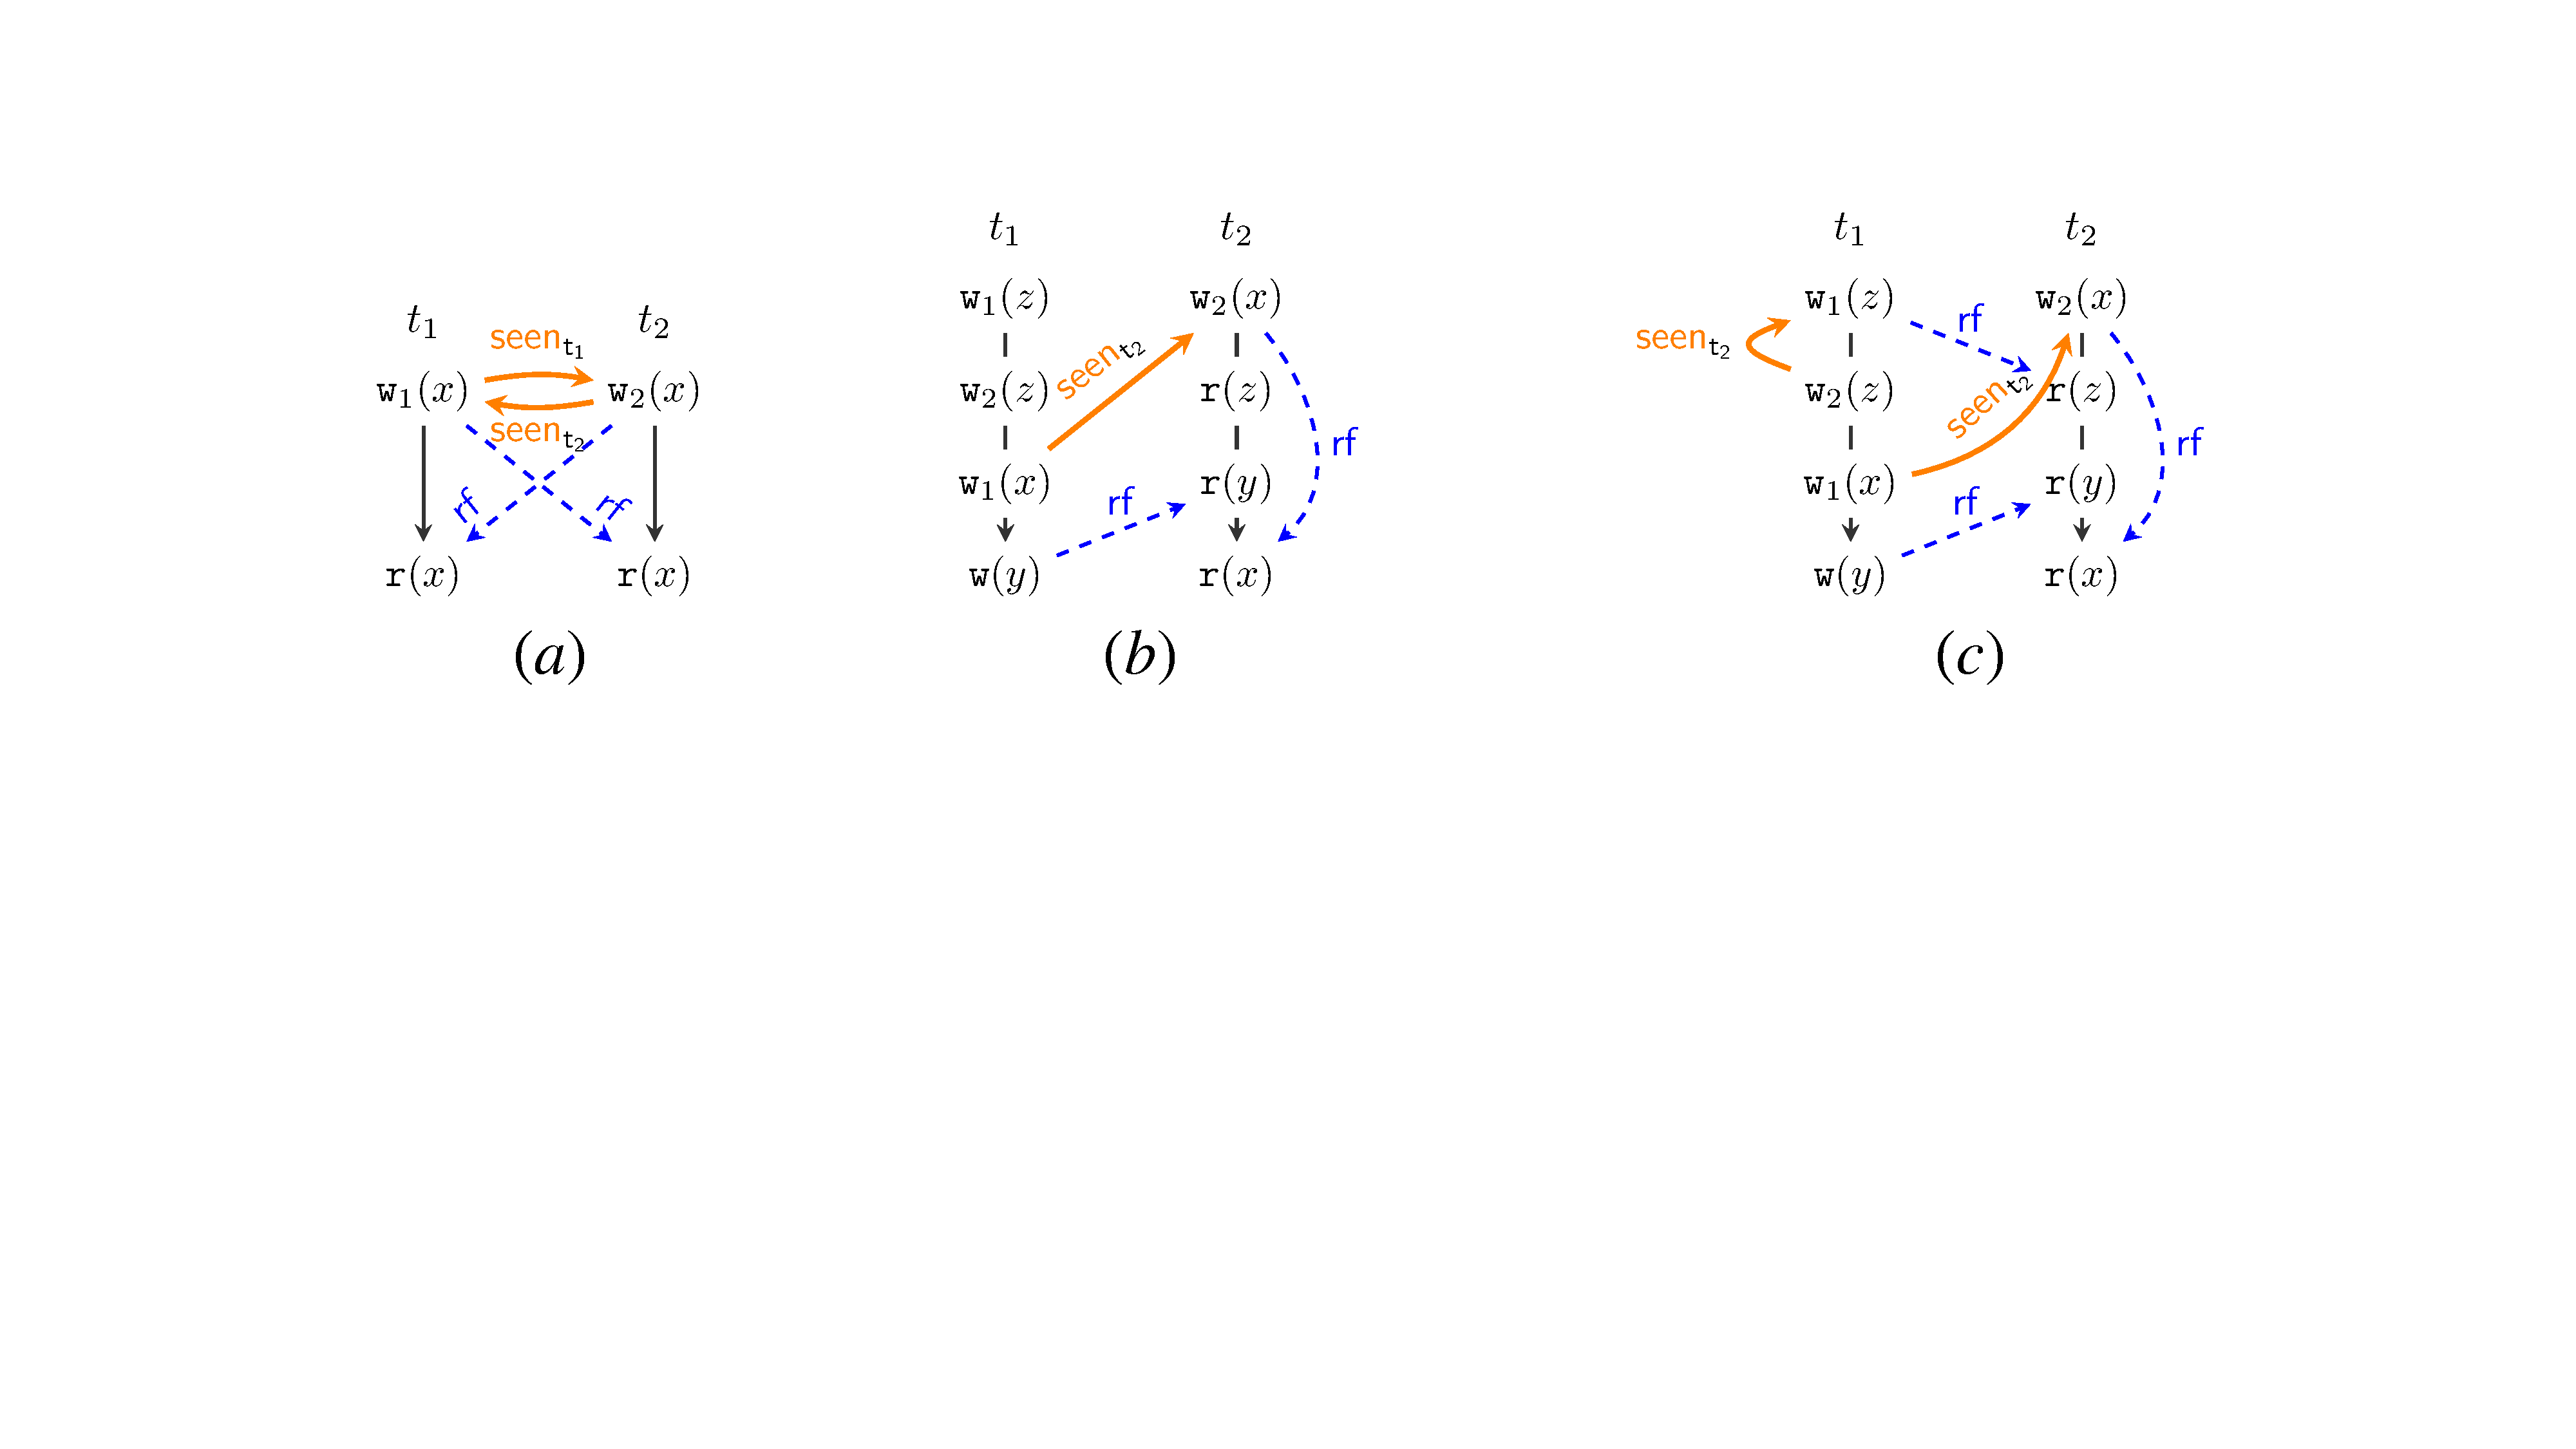
\includegraphics[width=\textwidth]{Figures/CM.pdf}
	\caption{(a) is $\cmmm$ consistent as $\ob{t_1}, \ob{t_2}$ are acyclic. 
	(b) is also $\cmmm$ consistent : the $\wt_1(x) \ob{t_2} \wt_2(x)$ is induced 
	by $\wt_1(x)~\hb~\rd(x)$ and $\wt_2(x)~\rf~\rd(x)$. 
	(c) is obtained 
	from (b) by adding $\wt_1(z)~\rf~\rd(z)$, and is $\cmmm$ inconsistent, 
since we have $\wt_1(z)~\po~\wt_2(z)~\ob{t_2}~\wt_1(z)$. 
	$\wt_2(z)~\ob{t_2}~\wt_1(z)$ is induced 
	from the conflicting triplet $(\wt_1(z), \rd(z), \wt_2(z))$ with 
	 $\wt_2(z)~\ob{t_2}~\rd(z)$. 
	}
	\label{cm:examples}
	\end{figure}

Since $\wramm=\ccmm$ and $\sramm=\cvmm$, both the fine-grained-hardness and $\NP$-hardness result for $\wramm, \sramm$ implies the same for  $\ccmm$ and $\cvmm$. So we only need to prove the hardness results for $\cmmm$.
In Section \ref{app:cc-1w}, we discuss the polynomial-time algorithm for \onewriter\ programs and in Section~\ref{app:cc-3w}, we discuss the complexity results for \threewriter\ programs under $\cmmm$. Note that the $\NP$-hardness for \twowriter\ programs under $\cmmm$ follows from arguments analogous to those made in Section~\ref{sec:hardness-twowriter} for RA models, and therefore we do not discuss it separately.

 	

For a $\cmmm$-consistent execution graph the following should be satisfied: $(\text{PORF})\land(\text{weak-Rcoh})\land (\text{\OB{}})$



 


\subsection{ \onewriter~ programs under Causal Consistency }~\label{app:cc-1w}

Recall that $\cmmm$ is essentially $\wramm$ with the extra axiom of $\ob{}$ acyclicity. We argue that the algorithm in  Section~\ref{sec:onewriter-algorithm} 
can be used for $\cmmm$ also. It is easy to see that any execution graph $\ex$  which is $\cmmm$-consistent is also $\wramm$-consistent. 


The other direction follows for the \onewriter{} case. 
Suppose $\ex$ is $\wramm$-consistent but  violates $\ob{t}$ acyclicity for some thread 
 $t$. Then we have  both $\wt'~\ob{t}~ \wt$ and  $\wt~\ob{t}~ \wt'$ for writes $\wt, \wt'$ on some location $x$. 
 
 By definition of $\ob{t}$, $\wt'~\ob{t}~ \wt$ implies the existence of a conflicting triplet $(\wt, \rd, \wt')$ such that 
   $\wt~\rf ~\rd$, $\wt'~\ob{t}~\rd$, $\rd~\po^?~ e_{max}$ where $e_{max}$ is the $\po$-maximal element of $t$.
  Likewise,  $\wt~\ob{t}~ \wt'$ implies the existence of a conflicting triplet $(\wt', \rd', \wt)$ such that 
   $\wt'~\rf ~\rd'$, $\wt~\ob{t}~\rd'$, $\rd'~\po^?~ e_{max}$ where $e_{max}$ is the $\po$-maximal element of $t$. 
      Since $\wt, \wt'$  are in the same thread, either $\wt~\po~\wt'$ or 
   $\wt'~\po~\wt$. Either way, we observe one violation for \WRCoh{} wrt $\rd$ or $\rd'$. 
   Thus, inconsistency wrt $\cmmm$ results in $\wramm$ inconsistency as well. 
    Therefore, the algorithm    for $\wramm$ can be employed for $\cmmm$ as well. 
   Thus in case of \onewriter~ the time complexity of consistency testing will be same as that of $\wramm$, $O(n^3)$. 
   
   Since $\cvmm = \sramm$ and $\ccmm=\wramm$, the lower bound result under BMM hypothesis in Section~\ref{sec:onewriter} holds for both $\cvmm$ and $\ccmm$. Finally, as mentioned previously,
for the single writer case, obtaining a cyclic $\ob{t}$ for a thread $t$ results in violation of \WRCoh{}.  In the reduction given in Section~\ref{sec:onewriter}, \WRCoh{} is violated in the presence of a triangle, hence, the result also holds for $\cmmm$.
   
   





\subsection{Fine-grained Hardness under ETH for \threewriter~ systems}~\label{app:cc-3w}


We will now discuss the fine-grained hardness of \threewriter -system under $\cmmm$. 
Since  $\cmmm$ is stronger than $\wramm$, the soundness part of the reduction in 
 Lemma \ref{lem:wra-eth}  follows : Assume $\expartial_\varphi^{\ramm} \models \cmmm$. Then 
 we know $\expartial_\varphi^{\ramm} \models \wramm$. Our soundness argument shows that 
 $\varphi$ is satisfiable. 
 
 For the completeness part, assume that $\varphi$ is satisfiable. We have already synthesized an $\rf, \mo$ which respect $\sramm$(and hence $\wramm$). We have to now show that, \OB{} is preserved by the synthesized $\rf$. 

\begin{lemma}\label{lem:eth-cm}
If $\varphi$ has a satisfying assignment, then $\expartial_\varphi^{\ramm} \models \cmmm$. 
\end{lemma}
\begin{proof}
Let $A$ be the satisfying assignment for $\varphi$. 
Say $A(x_i) = true$:

(i) For all pair of events in $\E$, $e~\hb~e'$ we have $e~\ob{T_F}~e'$

(ii) For the conflicting tiplet $(\tuple{T_i^0: \wt(s_i, 1)}, \tuple{T_f: \rd(s_i, 1)}, \tuple{T_i^1: \rd(s_i, 2)})$, we have $\tuple{T_i^1: \wt(s_i, 2)}~ \ob{T_f}~ \tuple{T_f: \rd(s_i, 1)}$ and $\tuple{T_f: \rd(s_i, 1)}~\po^?~e^{T_f}_{max}$ where $e^{T_f}_{max}$ is the $\po$-maximal event in $T_f$. This implies $\tuple{T_i^1: \wt(s_i, 2)}~\ob{T_f}~\tuple{T_i^0: \wt(s_i, 1)}$. 

As there are no $\hb$-cycle and no members of $\ob{T_f}$ directed from $T_i^0$ to $T_i^1$, $\ob{T_f}$ is irreflexive.

If we consider the relation $\ob{T_{\neg x_i}}$, for the conflicting triplet $(\tuple{T_i^0: \wt(v_i, 0)},\\ \tuple{T_{x_i}: \rd(v_i,0)}, \tuple{T_i^1: \wt(v_i, 1)})$ we have $\tuple{T_i^1: \wt(v_i, 1)}~\ob{T_{\neg x_i}}~\tuple{T_i^0: \wt(v_i, 0)}$. 

Again no members of $\ob{T_{\neg x_i}}$ are directed from $T_i^0$ to $T_i^1$. As there is no $\hb$-cycle, $\ob{T_{\neg x_i}}$ is also irreflexive. 

It is easy to see that $\ob{}$ is irreflexive for all remaining threads.
Hence \OB{} is preserved by the synthesized $\rf$

\end{proof}

\subsection{NP-hardness for \twowriter~ systems}

For \twowriter~ systems the reduction from 3-SAT instance has similar construction as that of $\wramm$ and the proof of the reduction will be on similar argument as the proof of the reduction for \threewriter.


